\documentclass[tikz,border=10pt]{standalone}
\usepackage{tikz}
\usetikzlibrary{arrows.meta,automata,positioning,shapes}

\begin{document}

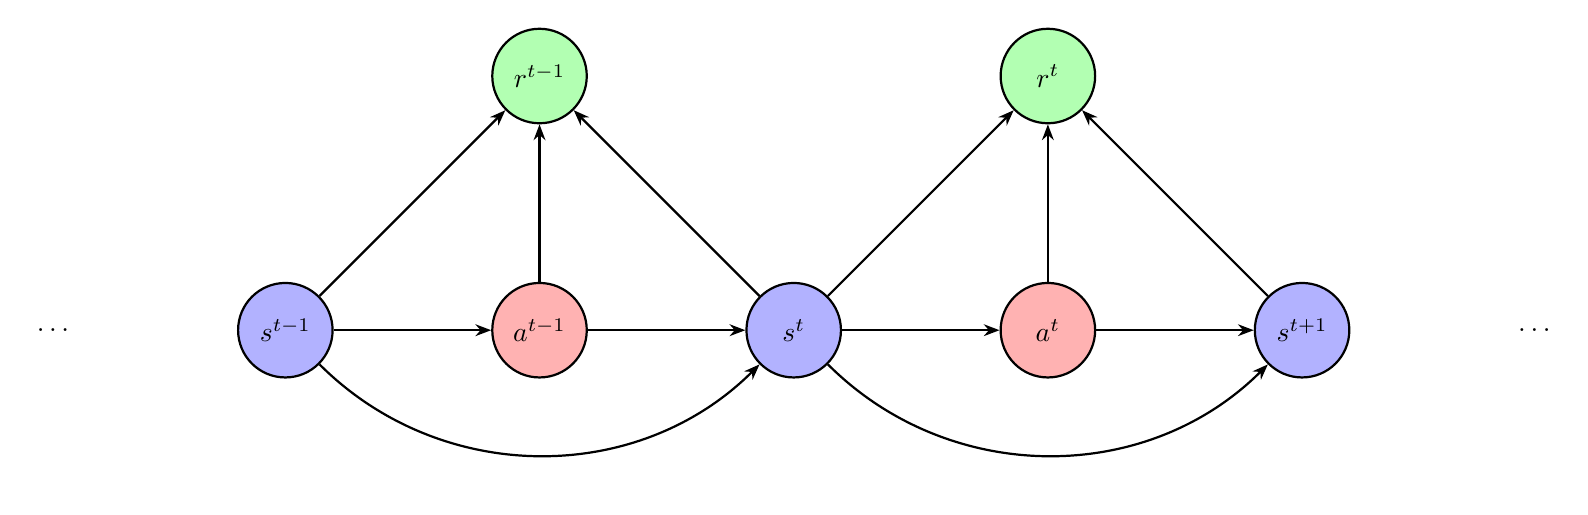
\begin{tikzpicture}[->, >={Stealth[length=2mm]}, node distance=2cm, thick, main/.style = {draw, circle, minimum size=1.2cm, align=center}]
  % Nodes
  \node[main, fill=blue!30] (s_t1) {\(s^{t-1}\)};
  \node[main, fill=red!30] (a_t1) [right=of s_t1] {\(a^{t-1}\)};
  \node[main, fill=blue!30] (s_t) [right=of a_t1] {\(s^t\)};
  \node[main, fill=red!30] (a_t) [right=of s_t] {\(a^t\)};
  \node[main, fill=blue!30] (s_t2) [right=of a_t] {\(s^{t+1}\)};

  \node[main, fill=green!30] (r_t1) [above=of a_t1] {\(r^{t-1}\)};
  \node[main, fill=green!30] (r_t) [above=of a_t] {\(r^t\)};

  Ellipses nodes
  \node (left_dots) [left=of s_t1] {\(\ldots\)};
  \node (right_dots) [right=of s_t2] {\(\ldots\)};

  % Paths

  % Paths
  \path 
        (s_t1) edge (a_t1)
        (s_t1) edge (r_t1)
        (a_t1) edge (s_t)
        (s_t) edge (a_t)
        (s_t) edge (r_t1)
        (s_t) edge (r_t)
        (a_t) edge (s_t2)
        (a_t1) edge (r_t1)
        (a_t) edge (r_t)
        (s_t2) edge (r_t)
        (s_t1) edge[bend right=45] (s_t)
        (s_t) edge[bend right=45] (s_t2);
\end{tikzpicture}

\end{document}


